\subsection{Links de aplicações}

Existem diferentes tipos de \textit{links} sendo que para \textit{mobile} é utilizado os \textit{app links}, \textit{deep links} e os \textit{dynamic links}.

Os \emph{app links} são "(...)\emph{web links that use the HTTP and HTTPS schemes}(...)"\citep{linking}, estes possuem também um atributo extra chamado \textit{autoVerify}. Este atributo permite a uma aplicação "(...)\emph{to designate itself as the default handler of a given type of link}(...)"\citep{linking}, isto permite que "(...)\emph{app opens immediately if it's installed}(...)"\citep{linking}. O grande problema é que estes \textit{links} não permitem o redirecionamento do utilizador para uma parte específica da aplicação e é necessário dispor de um domínio próprio.


Os \textit{deep links} são "(...)\emph{URIs of any scheme that take users directly to a specific part of your app}(...)"\citep{linking}, o grande problema deste tipo de \textit{links} é que se os utilizadores não dispuserem da aplicação instalada no dispositivo, este irá falhar e não permite a customização de comportamento.

Já os \textit{dynamic links}, desenvolvidos pela \textit{Firebase}, assim como os \textit{deep links} "(...)\emph{if a user opens a Dynamic Link on iOS or Android, they can be taken directly to the linked content in your native app}(...)"\citep{dynamic_linking}, mas para além disto, este permite que "(...)\emph{if a user opens the same Dynamic Link in a desktop browser, they can be taken to the equivalent content on your website}(...)"\citep{dynamic_linking}, ou seja, este permite a customização de comportamento de \textit{links} para diversas situações e em caso do utilizador não dispor da aplicação instalada, este permite que "(...)\emph{the user can be prompted to install it; then, after installation, your app starts and can access the link}(...)"\citep{dynamic_linking}. Visto que este é o comportamento desejado pelo cliente da aplicação, então foi decidido utilizar esta abordagem.

\begin{figure}[htb]
  \centering
  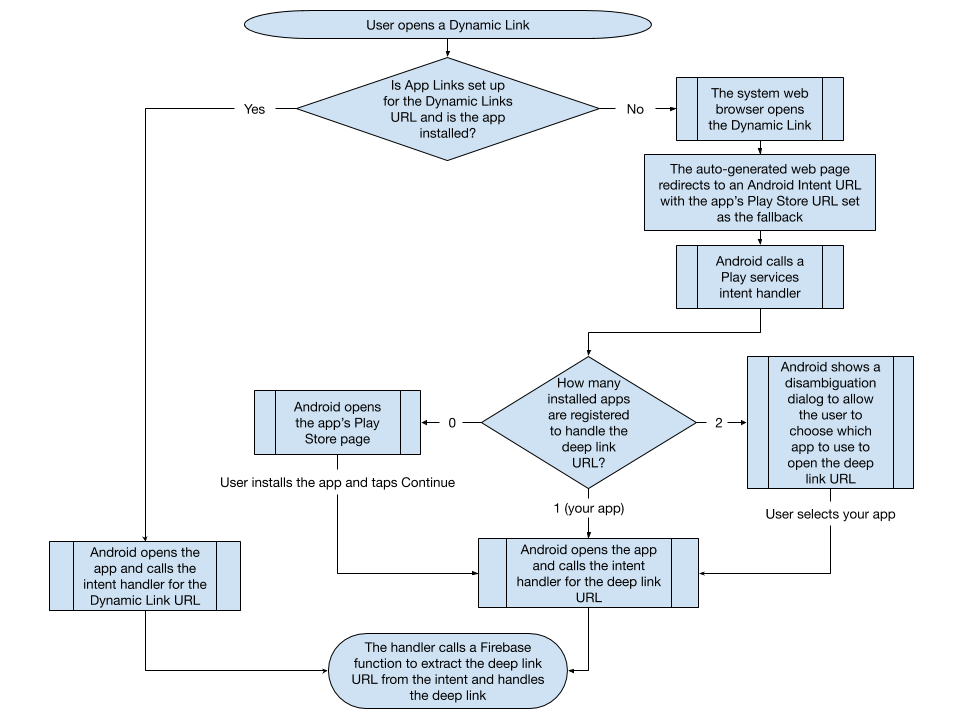
\includegraphics[width=0.83\textwidth]{images/diagramas/fdl-android-integration.png}
  \caption{Funcionamento dos dynamic links \citep{linking_firebase}}
  \label{fig:23}
\end{figure}
